%Hauptdokumentation der L�sung
\NeedsTeXFormat{LaTeX2e}

\documentclass[a4paper,oneside,abstract]{scrreprt}

\usepackage[left=2cm,right=2cm,top=1cm,bottom=2cm,includeheadfoot]{geometry}

\usepackage{ae}
\usepackage{ngerman}				% neue deutsche Rechtschreibung
\usepackage[ngerman]{babel}			% "Table of Contents" --> "Inhaltsverzeichnis"

\usepackage[T1]{fontenc}			% Fontkodierung auf T1-Format
\usepackage{graphicx}				% Bilder
\usepackage{fancyhdr}				% Kopf- und Fusszeilen
\usepackage{lastpage}				% Anzahl gesamte Seiten
\usepackage{hyperref}				% f\"ur Hyperlinks
\usepackage{array}					% f\"ur Tabellen (tabular Umgebung)
\usepackage{listings}				% Quellcodeausgabe
\usepackage{supertabular}			% f\"ur Tabellen \"uber mehrere Seiten
\usepackage{verbatim}	
\usepackage[applemac]{inputenc}
\usepackage{cite}
\usepackage{color}					% f�r Farben

% definition f�r Farben
\definecolor{LinkColor}{rgb}{0,0,0.5}
\hypersetup{
	colorlinks=true,				% definition der Links im PDF
	linkcolor=LinkColor,
	citecolor=LinkColor,
	filecolor=LinkColor,
	menucolor=LinkColor,
	pagecolor=LinkColor,
	urlcolor=LinkColor
}


\newcommand{\titel}{Spektrometer App}
\newcommand{\doctype}{Bachelor Thesis}
\newcommand{\untertitel}{Anbindung Spektrometer an mobiles Device}
\newcommand{\datum}{\today}
\newcommand{\autorA}{Andreas L�scher}
\newcommand{\autorB}{Raphael Bolliger}
\newcommand{\ort}{Windisch}
\newcommand{\dozent}{Martin Gwerder}
\newcommand{\auftraggeber}{Andreas Hueni}

\title{\titel}
\author{\autorA  \and \AutorB}
\date{\datum}

\pagestyle{fancy}

\fancyhf{}

\fancypagestyle{plain}{
	
	\fancyhf{}
	
	\fancyhead[R]{\nouppercase{\leftmark}}
	
	\fancyfoot[L]{\doctype}	
	\fancyfoot[C]{Seite \thepage\ von \pageref{LastPage}}
	\fancyfoot[R]{\titel}
	
	\renewcommand{\footrulewidth}{0.5pt}	% Trennlinie Fusszeile
	\renewcommand{\headrulewidth}{0.5pt} 	% obere Trennlinie
	
	\renewcommand{\headwidth}{17cm} 		% Breite der Kopf- und Fusszeile (21cm-2*2cm)
}

\begin{document}

\parindent 0pt							% kein Einzug bei 1. Zeile eines paragraphs
\parskip 5pt							% 5pt Abstand zwischen den einzelnen Abs�tzen						% Seitenr�nder, Kopf-/Fusszeilen, usw.

% Titelseite
\thispagestyle{plain}

\begin{titlepage}
	\begin{center}
		\vspace*{1cm}
		\textbf{
			\hspace{-0.12cm}\LARGE{\doctype}\\
			\Huge{\titel}\\
			\vspace{0.5cm}
			\large{\untertitel}\\
			\vspace{1.5cm}
			\large{\autorA, \autorB}\\
		}
		
		\begin{center}
		\vspace*{0.5cm}
		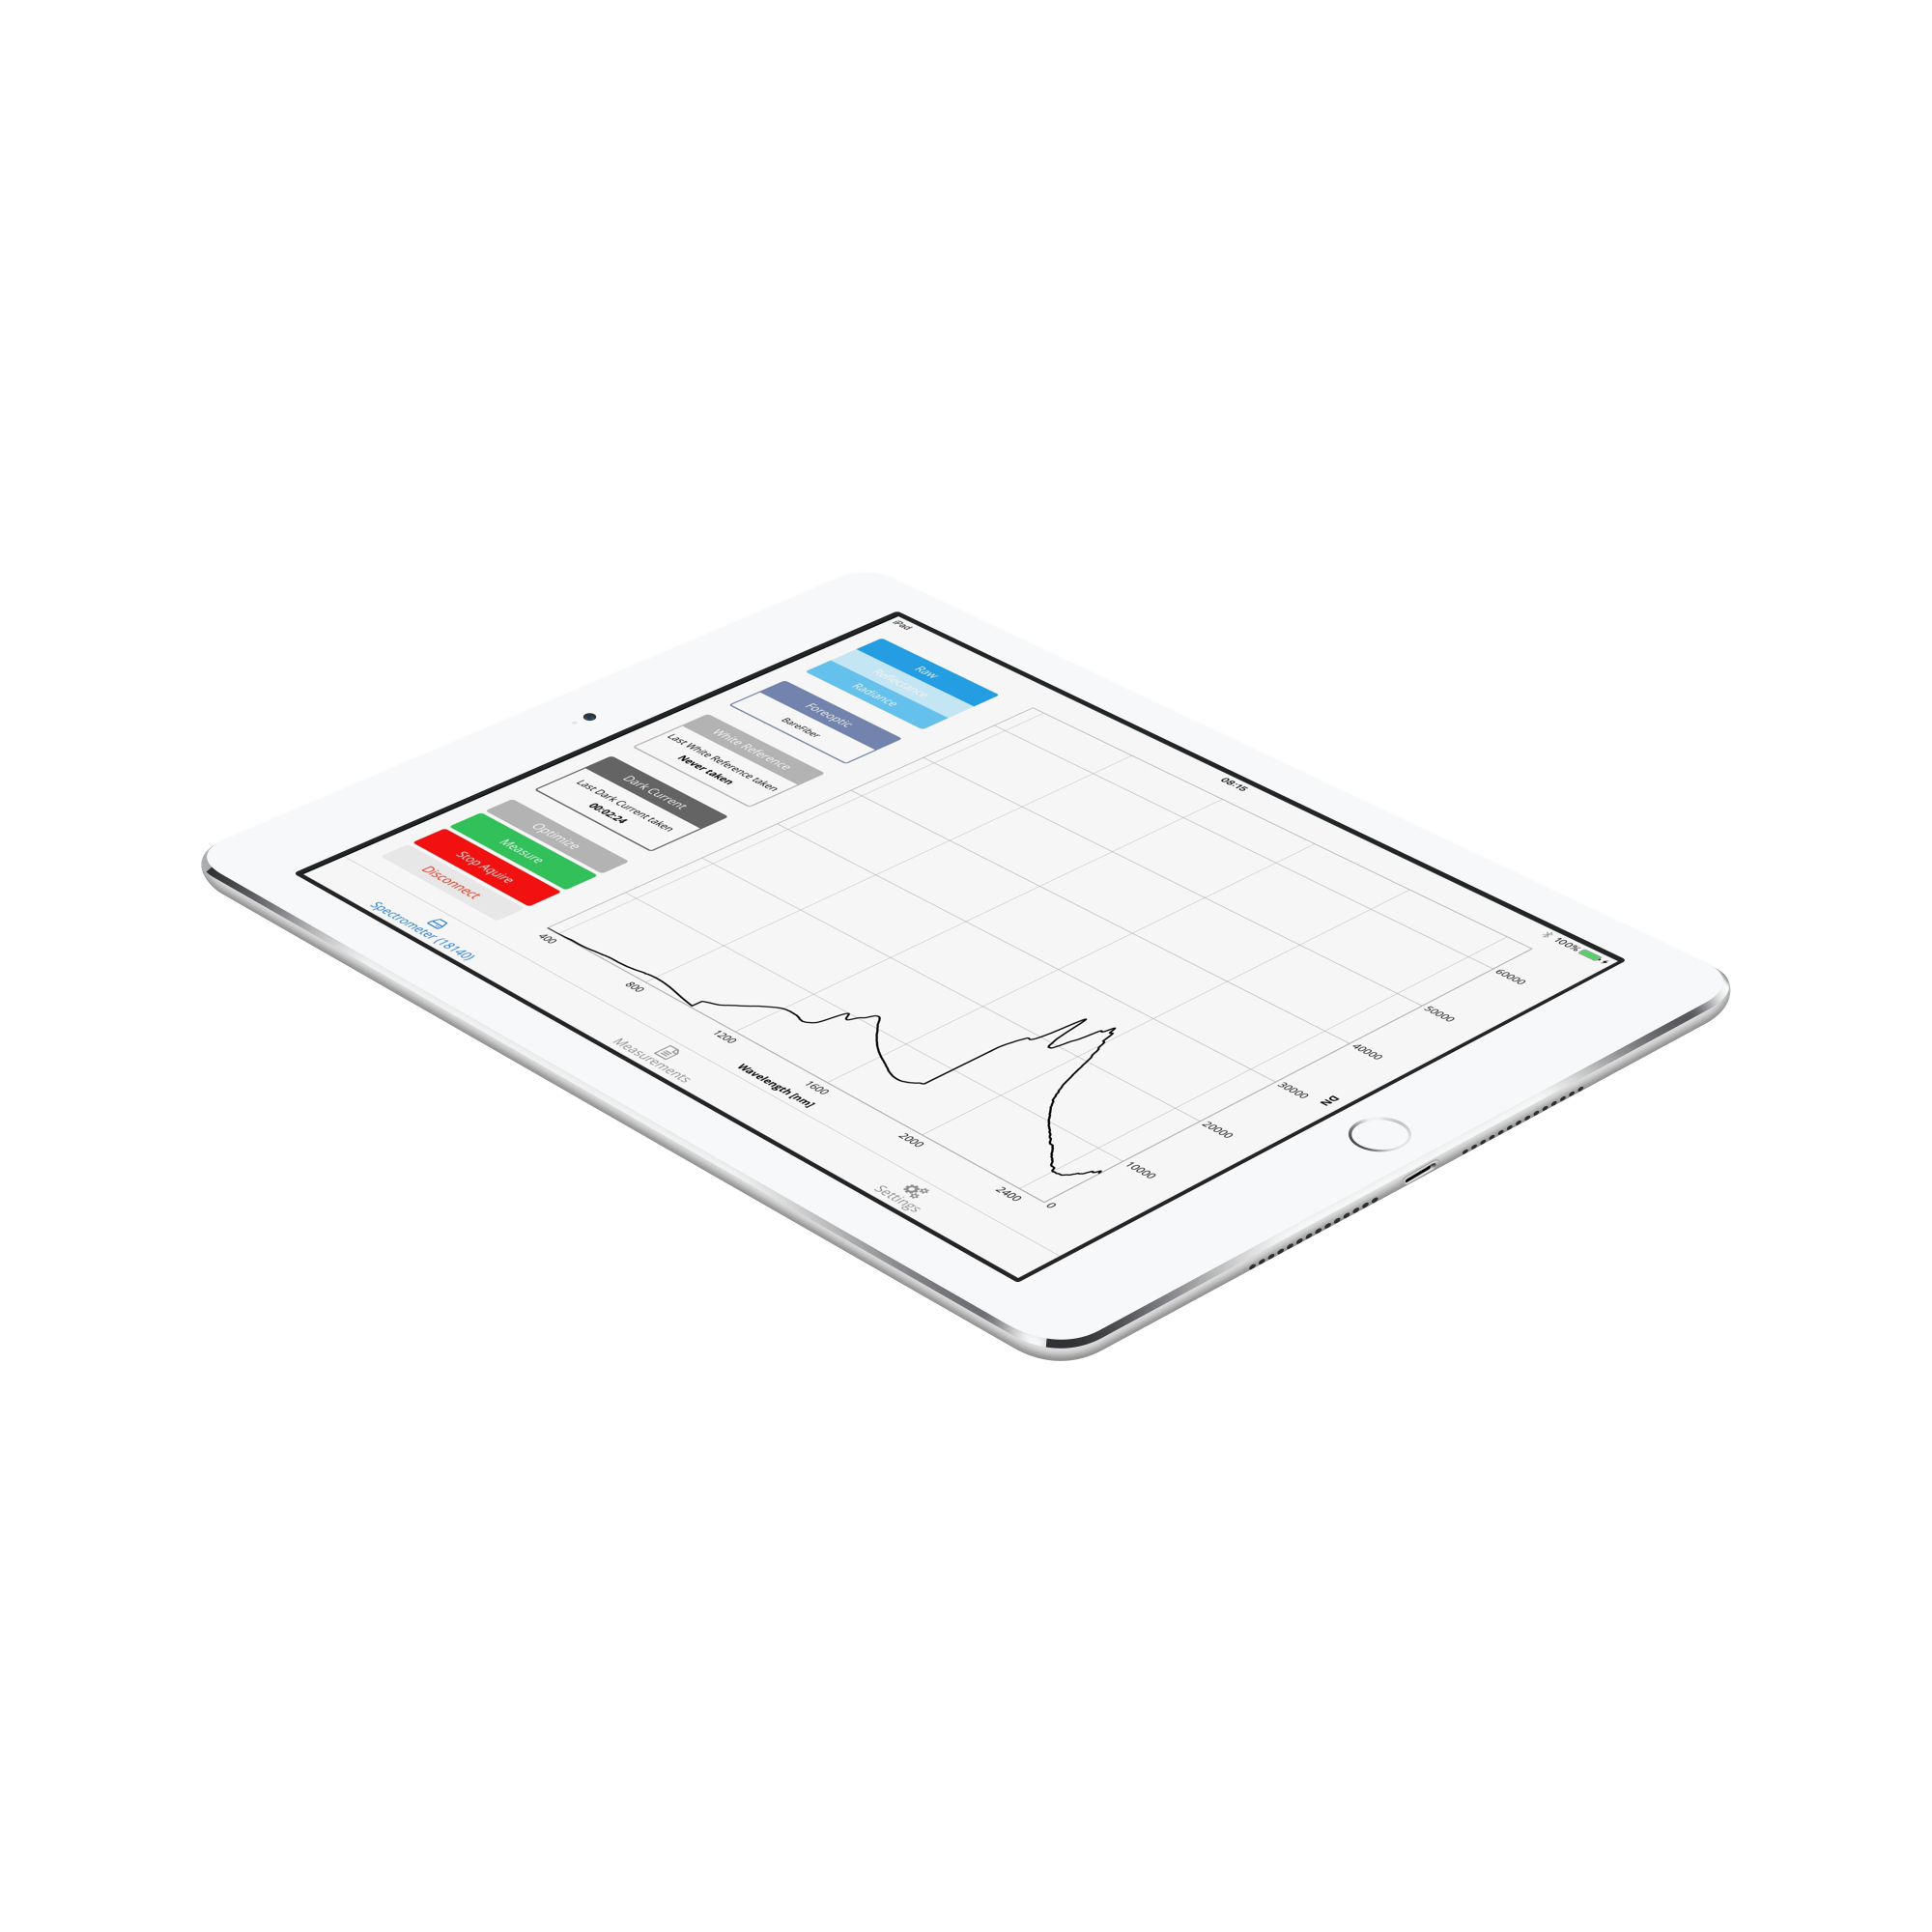
\includegraphics[scale=0.3]{images/ipadAir_Spektrometer}
		\end{center}
		
		\vfill
		\large{
			\hspace{-0.83cm} 
\includegraphics{images/fhnw_logo}\\
			\line(1,0){165}	

			\vspace{0.5cm}
			Dozent: \dozent \\
			\vspace{0.1cm}
			Auftraggeber:  \auftraggeber \\
			\vspace{0.5cm}
			\ort, \datum
		}
	\end{center}
\end{titlepage}

% Inhaltsverzeichnis
\tableofcontents
\listoffigures 								% Abbildungsverzeichnis

% Abstract
\begin{abstract}

Das Hauptziel des Projektes ist, eine mobile Applikation zu erstellen, welche die RS\textsuperscript{3} Desktopl�sung von ASD abl�st. RS\textsuperscript{3} ist eine Software, welche die Verbindung zu einem Spektralmessger�t herstellt, Messungen ausl�sen sowie die Resultate anzeigen kann. Das bisherige System besteht aus einem Laptop inklusive RS\textsuperscript{3} Software, welche jeweils auf ein Spektrometer abgestimmt ist. Neu soll eine mobile App ausreichen, um mehrere Spektrometer ansprechen zu k�nnen. Die App soll Forschende unterst�tzen, Messungen direkt im Feld zu beurteilen und verwalten zu k�nnen. Die erstellten Messungen sollen abschliessend exportiert werden k�nnen, um diese am Computer weiterzuverwenden. 

\end{abstract}
\pagenumbering{arabic}

% Ausgangslage und Problemstellung
\chapter{Einleitung}

\section{Ziel der Arbeit} \label{ziel}
Das geologische Institut der Universit�t Z�rich betreibt zur Forschung vier Spektrometer der Firma ASD Inc. aus Colorado in den USA. Zu jedem Spektrometer liefert ASD einen Notebook mit installierter Software, um das  \gls{spectrometer} zu bedienen und Messungen auszuf�hren.

Ziel dieser Arbeit war, die Software \href{https://www.asdi.com/products-and-services/software/rs3}{RS\textsuperscript{3}} von ASD mit einer modernen Applikation f�r ein mobiles Device abzul�sen. Das Projektteam hat sich gemeinsam mit dem Kunden dazu entschieden, die Applikation f�r iOS Ger�te, im speziellen iPads, zu entwickeln.

\section{Hilfestellungen} \label{hilfestellungen}
Zur Umsetzung konnten verschiedene Hilfestellungen in Anspruch genommen werden. ASD bietet auf ihrer Webseite einen \href{http://support.asdi.com/Products/Products.aspx}{Download} mit einem Developer-Kit an. In dieser Dokumentation ist beschrieben, wie interessierte Entwickler mittels eines TCP-Servers, der auf dem Spektrometer betrieben wird, selbst Applikationen entwickeln k�nnen. Die Dokumentation enth�lt ausf�hrliche Informationen zu Verbindungsparameter, R�ckgabetypen und Dateiformaten.

Weiter konnte auf das \href{https://github.com/ahueni/SPECCHIO}{GitHub Repository} der SPECCHIO-Datenbank zur�ckgegriffen werden. In dieser Applikation wurden verschiedenste Berechnungen und Manipulationen mit Spektraldaten oder Spektraldateien bereits in Java programmiert.

\section{Erreichtes} \label{erreichtes}
Die Applikation wurde mit den definierten Grundanforderungen vollst�ndig umgesetzt. Der Benutzer kann, sofern das iPad mit dem Spektrometer �ber WLAN verbunden ist, das Spektrometer bedienen und Messungen ausf�hren. Es wurde speziell darauf geachtet, den Messablauf einfacher und f�r den Benutzer intuitiver zu gestalten. Die Grundansicht wurde nahezu von der bestehenden Software �bernommen. Somit sollte es f�r die Benutzer keine zu grosse Umstellung sein.

Weiter wurde darauf geachtet, die Applikation in Zukunft noch weiter zu entwickeln. Die Architektur wurde stark strukturiert, damit auch Personen, die noch nicht mit dem Projekt vertraut sind, eine Weiterentwicklung vornehmen k�nnen. 

\section{Leserf�hrung} \label{leserfuehrung}
Dieses Dokument beschreibt die Erarbeitung eines Informatik Projektes 6 der Fachhochschule Nordwestschweiz. Die Dokumentation ist in einen theoretischen und einen praktischen Teil aufgeteilt. Im theoretischen Teil wird nur kurz erkl�rt was ein Spektrometer genau misst und wie die Daten berechnet und abgespeichert werden. Im praktischen Teil wird vor allem die Softwarearchitektur und die konkrete Umsetzung genau beschrieben.


% Benutzung
\chapter{Bentzung}

\section{}

\section{UI}

% Umsetzung
\chapter{Umsetzung}
Dieses Kapitel beschreibt die Umsetzung des Produktes.
Die Nachfolgenden Abschnitte werden Schrittweise detaillierter und beschreiben den Aufbau sowie die Designentscheidungen des Softwarecodes.

\section{Einleitung}
\section{Anforderungen}
\section{Technologien}
In diesem Abschnitt wird beschrieben, welche Technologien und Tools eingesetzt wurden, um die iOS Applikation umzusetzen. Es wurde darauf geachtet, dass bew�hrte und von den Herstellern vorgesehene Technologien verwendet wurden.
\subsection{Entwicklungsumgebung}
Das Projekt wurde mit XCode 8.2.1 umgesetzt. Grunds�tzlich, kann jede IDE verwendet werden, welche mit Swift kompatibel ist. Um das Projekt builden zu k�nnen wird zwingend ein Apple Rechner ben�tigt.
\subsection{Programmiersprache}
Das Projekt wurde in der Programmiersprache Swift 3 umgesetzt und ist mit iOS 10 und h�her kompatibel. Es wurde darauf geachtet, dass alle Abh�ngigkeiten ebenfalls in Swift umgesetzt sind. Dies erleichtert die Weiterentwicklung da kein, f�r unge�bte Entwickler, meist schwer lesbarer Objective C Code zum Einsatz kommt.
\subsection{Abh�ngigkeiten}
Externe Ressourcen, wurden vorwiegend mit CocoaPods eingebunden. CocoaPods ist ein Packet Manager, mit welchem man Packete in ein bestehendes Projekt einbinden kann. Dies geschieht �ber ein sogenanntes Podfile, welches zum Projektumfang geh�rt. Dieses File beschreibt die externen Abh�ngigkeiten, sowie welche Version ben�tigt wird.

Folgende Pods wurden f�r das Projekt verwendet:
\begin{itemize}
\item	 pod 'Charts/Realm'
\item    pod 'Zip'
\item    pod 'PlainPing'
\item    pod 'Pulsator'
\item    pod 'FontAwesome.swift'
\end{itemize}
    
Einzig die TCP Kommunikation wurde mit externem Code gel�st, welcher nicht als Pod verf�gbar ist.
\section{Architektur}

\subsection{Grobarchitektur}
Um weite Teile des Sourcecodes erneut nutzen zu k�nnen, wurde das Projekt in drei Teile aufgeteilt. Diese 3 Teile werden in den folgenden Abschnitten beschrieben.

\subsection{Core}
Der Core Ordner fasst den gesamten Code zusammen, welcher Platformunabh�ngig ist. Dieser Code kann auch in anderen Projekten mit �hnlicher Anwendung benutzt werden.
\subsection{Service}
Der Service Layer, kapselt einige Anfragen des App Layers an den Core Teil. Dieser Layer wird oft dazwischen gelegt, um beispielsweise Parallelit�t zu vermeiden. So wird im Layer beispielsweise ein Synchronized Queue ben�tigt, um nur ein Request nach dem Anderen an ein Spektrometer zu senden.
\subsection{iOS App}
Dieser Layer beinhaltet die eigentliche iOS App mit all Ihren typischen Eigenschaften, wie das AppDelegate und die Storyboards. In diesem Ordner werden alle Views sowie deren Controller gespeichert.

\section{Core}
\subsection{Connection}
In diesem Ordner, befindet sich die TCPManager Klasse sowie die externen Socks Dateien. Das Socks Framework k�mmert sich um die Kommunikation auf TCP Ebene. Eine ausf�hrliche Dokumentation ist unter folgendem Link zu finden: 
\newline
https://github.com/vapor/socks
\newline
Der TCP Manager ist f�r die Anfragen des Ger�tes verantwortlich. Es ist die einzige Klasse, welche direkt mit dem Spektrometer kommuniziert. Er ist deshalb auch als Singleton umgesetzt. Mit der connect Funktion, kann eine Verbindung zum ASD Ger�t hergestellt werden, danach k�nnen beliebig viele Kommandos mit sendCommand gesendet werden. Um die Verbindung zu schliessen, muss lediglich die disconnect Methode aufgerufen werden.

\subsection{Input/Output}
In diesem Kapitel, werden alle Klassen beschrieben, welche direkt Daten einlesen oder Ausgeben.
\subsubsection{File Writer}
Die Output Klassen, dienen dazu ein Indico File zu schreiben. Die Base Klasse kapselt daf�r alle Schreibvorg�nge. Von der Klasse File Writer, wird auf diese Methoden zugegriffen und st�sst so das Schreiben in der Richtigen Reihenfolge an.
\subsubsection{File Reader}
\subsubsection{Spectrometer Parser}

\subsection{Calculations}
\subsection{Error Handling}

\section{Service}

\subsection{Instrument Store}
\subsection{Command Manager}
\subsection{File Write Manager}

\section{iOS App}
\subsection{App Delegate}
\subsection{Core Data}
\subsection{Views}

Alle ViewController sind in der Datei Main.storyboard enthalten. Dies war eine bewusste Entscheidung, um Entwicklern einen guten �berblick �ber den gesamten UI Ablauf zu erm�glichen. Einzig das Design f�r eine Zelle der Mess�bersichtstabelle wurde in eine eigne XIB-Datei ausgelagert.

Die Anordnung der Controls wurde im Storyboard gel�st. Kleinere Merkmale wurden jeweils im Code angepasst, indem von bestehenden Controls abgeleitet wurde.

\subsection{Controllers}

\subsubsection{Settings}

Einstellungen, welche pro Applikation verf�gbar sein m�ssen, werden in den sogenannten UserDefaults gespeichert. Dieser Speicher, kann s�mtliche serialisierbaren Objekte speichern.

\subsection{Components}
\subsection{View Store}
\subsection{Service}
\subsubsection{Validation}

F�r die Validierung wurde von jedem benutzen Control eine Ableitung erstellt und und das BaseValidationControl Protokoll implementiert. Dieses Protokoll enth�lt ein Property isValid welches den G�ltikeitszustand des Objektes enth�lt.

In jedem ViewController, muss nun nur noch der ValidationManager aufgerufen werden und die Hauptview �bergeben werden. Dieser ValidationManager pr�ft nun alle Subviews, welchedas Protokoll implementieren.

Um die Validation f�r einen neuen ViewController hinzuzuf�gen, kann folgendermassen vorgangen werden:
1. Erstellen Sie einen neuen ViewController
2. F�gen Sie ein Control hinzu und leiten sie von einem bestehenden ValidationControl ab. Oder erstellen Sie eine neue Ableitung eines Controls und implementieren Sie das BaseValidationControl Protokoll.
3. Rufen Sie die validateSubViews Methode des ValidationMangers auf.


\subsubsection{File Browser}

\end{document}